\documentclass[12pt]{article}
\usepackage[utf8]{inputenc}
\usepackage{polski}
\usepackage{listing}
\usepackage{listings}
\usepackage{amsmath}
\usepackage{multicol}
\usepackage{graphicx}
\usepackage[shortlabels]{enumitem}
\usepackage{amssymb}
\usepackage{algorithmic}
\usepackage{algorithm}
\graphicspath{ {./images/} }
\title{
	Obliczenia naukowe \\
	Sprawozdanie 5
}
\addtolength{\oddsidemargin}{-.8in}
\addtolength{\evensidemargin}{-.8in}
\addtolength{\textwidth}{1.75in}
\addtolength{\topmargin}{-.7in}
\addtolength{\textheight}{1.75in}

\floatname{algorithm}{Algorytm}

\date{29 grudnia 2019}
\author{Józef Piechaczek}

\begin{document}

\pagenumbering{gobble}
\maketitle
\newpage
\pagenumbering{arabic}

\setlength{\abovedisplayskip}{5pt}
\setlength{\belowdisplayskip}{5pt}

\section*{Opis problemu}
W zadaniu mamy do czynienia z problemem rozwiązania układu równań liniowych
\begin{equation*}
	Ax = b
\end{equation*}
dla danej macierzy współczynników $\textbf{A} \in \mathbb{R}^{n \times n}$ i wektora prawych stron $b \in \mathbb{R}^n, n \geq 4$ Macierz $\textbf{A}$ jest rzadką i blokową o następującej strukturze:
\begin{equation}
A = 
\begin{pmatrix}
\textbf{A}_1 & \textbf{C}_1 & \textbf{0} & \textbf{0} & \textbf{0} & \cdots & \textbf{0} \\
\textbf{B}_2 & \textbf{A}_2 & \textbf{C}_2 & \textbf{0} & \textbf{0} & \cdots & \textbf{0} \\
\textbf{0} & \textbf{B}_3 & \textbf{C}_3 & \textbf{A}_3 & \textbf{0} & \cdots & \textbf{0} \\
\vdots & \ddots & \ddots & \ddots & \ddots & \ddots & \vdots \\
\textbf{0} & \cdots & \textbf{0} & \textbf{B}_{v-2} & \textbf{A}_{v-2} & \textbf{C}_{v-2} & \textbf{0} \\
\textbf{0} & \cdots & \textbf{0} & \textbf{0} & \textbf{B}_{v-1} & \textbf{A}_{v-1} & \textbf{C}_{v-1} \\
\textbf{0} & \cdots & \textbf{0} & \textbf{0} & \textbf{0} & \textbf{B}_{v} & \textbf{A}_{v} \\
\end{pmatrix}
\end{equation}
$v = n/\ell$, zakładając, że $n$ jest podzielne przez $\ell$, gdzie $\ell \geq 2 $ jest rozmiarem wszystkich kwadratowych macierzy wewnętrznych (bloków) $\textbf{A}_k$, $\textbf{B}_k$ i $\textbf{C}_k$. Mianowicie, $\textbf{A}_k \in \mathbb{R}^{\ell \times \ell}, k = 1, \dots, v$ jest macierzą gęstą, $\textbf{0}$ jest kwadratową macierzą zerową stopnia $\ell$, macierz $\textbf{B}_k \in  \mathbb{R}^{\ell \times \ell}, k = 2, \dots, v$ jest następującej postaci:
\begin{equation}
\textbf{B}_k = 
\begin{pmatrix}
0 & \cdots & 0 & b^k_{1 \ell-1} & b^k_{1 \ell} \\
0 & \cdots & 0 & b^k_{2 \ell-1} & b^k_{2 \ell} \\
\vdots & & \vdots & \vdots & \vdots \\
0 & \cdots & 0 & b^k_{\ell \ell-1} & b^k_{\ell \ell} \\
\end{pmatrix}
\end{equation}
$\textbf{B}_k$ ma tylko dwie ostatnie kolumny niezerowe. Natomiast  $\textbf{C}_k \in \mathbb{R}^{\ell \times \ell}, k = 1, \dots, v-1$ jest macierzą diagonalną:
\begin{equation}
\textbf{C}_k = 
\begin{pmatrix}
c^k_1 & 0 & 0 & \cdots & 0 \\
0 & c^k_2 & 0 & \cdots & 0 \\
\vdots & \ddots & \ddots & \ddots & \vdots \\
0 & \cdots & 0 & c^k_{\ell - 1} & 0 \\
0 & \cdots & 0 & 0 & c^k_{\ell}\\
\end{pmatrix}
\end{equation}
Macierz $\textbf{A}$ jest bardzo dużego rozmiaru ($n$ jest bardzo duże) co wyklucza pamiętanie macierzy jako dwuwymiarowej tablicy oraz użycie standardowych (bibliotecznych) algorytmów dla macierzy gęstych. Należy zatem użyć specjalnej struktury pamiętającej efektywnie macierz $\textbf{A}$, która pamięta tylko elementy niezerowe oraz zaadaptować algorytmy tak, aby uwzględniały specyficzną postać macierzy. Zakładając, że $\ell$ jest stałe, czas rozwiązywania układu powinien zostać zredukowany do $O(n)$.

%\section*{Opis funkcji dodatkowych}
%Programy umożliwiają czytanie danej macierzy $\textbf{A}$ i wektora prawych stron $\textbf{b}$ z plików tekstoeych, 

\section{Zadanie 1}
Zadanie 1 polega na napisaniu funkcji rozwiązującej układ $Ax = b$ metodą eliminacji Gaussa z uwzględnieniem specyficznej postaci macierzy $\textbf{A}$ dla dwóch wariantów:
\begin{enumerate}[(a)]
	\item bez wyboru elementu głównego,
	\item z częściowym wyborem elementu głównego.
\end{enumerate}

\subsubsection*{Metoda eliminacji Gaussa}
Metoda eliminacji Gaussa to algorytm rozwiązywania układów liniowych i wyznaczania rozkładu \textbf{LU} wykorzystujący trzy typy operacji elementarnych:
\begin{enumerate}[(a)]
	\item Zamiana dwóch wierszy
	\item Mnożenie wiersza przez element niezerowy
	\item Dodawanie wielokrotności jednego rzędu do innego
\end{enumerate}
Za pomocą tych operacji jesteśmy w stanie zamienić macierz do postaci trójkątnej górnej. Algorytm polega na używaniu operacji elementarnych w ten sposób, aby w danej iteracji pod wartością na diagonali znajdowały się tylko wartości 0. W tym celu od wierszy znajdujących się poniżej rozpatrywanego odejmujemy taką wielokrotność rozpatrywanego rzędu, aby wyzerować wartość w rozpatrywanej kolumnie. Gdy macierz znajduje się w postaci trójkątnej górnej możemy użyć algorytmu \textit{podstawienia wstecz} do łatwego rozwiązania układu. Algorytm \textit{podstawienia wstecz} polega na rozpoczęciu rozwiązywania układu od dołu układu, gdzie uzyskujemy równanie $a_n x_n = b_n$, zatem $x_n = b_n/a_n$, następnie poprzednio uzyskane rozwiązana używamy do rozwiązania równania znajdującego się wyżej, gdzie obliczamy kolejną wartość $x_i$. Algorytm kończy się, gdy przejdziemy po wszystkich wierszach.
Standardowy algorytm zamiany do postaci trójkątnej górnej ma złożoność czasową $O(n^3)$, a algorytm \textit{podstawienia wstecz} $O(n^2)$, co daje łączny czas $O(n^3)$.

\begin{algorithm} % enter the algorithm environment
\caption{Metoda Gaussa}
\label{alg1} % and a label for \ref{} commands later in the document
\begin{algorithmic} % enter the algorithmic environment
    \REQUIRE $n, (a_{ij}), b_i$
    \STATE \{\textbf{Pętla 1}\}
    \FOR{$k=1$ \textbf{to} $n-1$}
    		\STATE \{\textbf{Pętla 2}\}
		\FOR{$i=k+1$ \textbf{to} $n$}
		\STATE $z \leftarrow a_{ik}/a_{kk}$
		\STATE $a_{ik} \leftarrow 0$
    			\STATE \{\textbf{Pętla 3}\}
			\FOR{$j=k+1$ \textbf{to} $n$}
				\STATE $a_{ij} \leftarrow a_{ij} - z a_{kj}$
    			\ENDFOR
    			\STATE $b_i \leftarrow b_i - z b_k$
    		\ENDFOR
    \ENDFOR
    \STATE \{\textbf{Pętla 4}\}
    \FOR{$i=n$ \textbf{to} $1$ \textbf{step} $-1$}
		\STATE $x_i \leftarrow (b_i - \sum^n_{j=i+1}a_{ij}x_j)/a_{ii}$
    \ENDFOR
\end{algorithmic}
\end{algorithm}

\subsubsection*{Metoda eliminacji Gaussa z częściowym wyborem elementu głównego}
Metoda eliminacji Gaussa z częściowym wyborem elementu głównego zawiera jedną modyfikację w porównaniu do tradycyjnego algorytmu. Na początku każdej iteracji zewnętrznej pętli algorytmu szukamy wiersza, który zaczyna się od bezwzględnie największej wartości, a następnie zamieniamy ten wiersz z aktualnie rozpatrywanym. Umożliwia to rozwiązanie układu, gdy na diagonali pojawią się zera. Zamiana wierszy w praktyce może okazać się kosztowną operacją, dlatego w algorytmie stosujemy tablicę $\textbf{p}$, początkowo zawierającą wartości od $1$ do $n$. W momencie, gdy powinniśmy zamienić wiersze, zamieniamy odpowiadające im wartości w tabeli $\textbf{p}$. Za każdym razem gdy odnosimy się do określonego wiersza używamy wartości z tabeli $\textbf{p}$.

\begin{algorithm} % enter the algorithm environment
\caption{Metoda Gaussa z częściowym wyborem elementu głównego}
\label{alg2} % and a label for \ref{} commands later in the document
\begin{algorithmic} % enter the algorithmic environment
    \REQUIRE $n, a_{ij}), b_i$
    \STATE $p \leftarrow [n]$
    \STATE \{\textbf{Pętla 1}\}
    \FOR{$k=1$ \textbf{to} $n-1$}
		\STATE wybór takiego $j \geq k$, że $|a_{p_jk}| \geq |a_{p_kk}|$
		\STATE $p_j \leftrightarrow p_k$
    		\STATE \{\textbf{Pętla 2}\}
		\FOR{$i=k+1$ \textbf{to} $n$}
		\STATE $z \leftarrow a_{p_ik}/a_{p_kk}$
		\STATE $a_{p_ik} \leftarrow 0$
    			\STATE \{\textbf{Pętla 3}\}
			\FOR{$j=k+1$ \textbf{to} $n$}
				\STATE $a_{p_ij} \leftarrow a_{p_ij} - z a_{p_kj}$
    			\ENDFOR
    			\STATE $b_{p_i} \leftarrow b_{p_i} - z b_{p_k}$
    		\ENDFOR
    \ENDFOR
    \STATE \{\textbf{Pętla 4}\}
    \FOR{$i=n$ \textbf{to} $1$ \textbf{step} $-1$}
		\STATE $x_i \leftarrow (b_{p_i} - \sum^n_{j=i+1}a_{p_ij}x_j)/a_{p_ii}$
    \ENDFOR
\end{algorithmic}
\end{algorithm}

\subsubsection*{Zmodyfikowany algorytm}
Analizując specyficzną budowę macierzy $\textbf{A}$ możemy dostrzec, że nie jest konieczne iterowanie po wszystkich wierszach dla \textbf{pętli 2}, ponieważ poniżej pewnego wiersza, dla danej kolumny, będą się znajdować wyłącznie elementy zerowe. Możemy dostrzec, że indeks wiersza ostatniego elementu niezerowego w danej kolumnie uzależniony jest od wielkości bloków w macierzy $\textbf{A}$ oraz od aktualnie rozpatrywanego elementu. Dla pierwszych $\ell - 2$ kolumn indeksem najniżej położonego niezerowego elementu jest ostatni wiersz macierzy $\textbf{A}_1$. Dla kolejnych $\ell$ kolumn indeksem najniżej położonego niezerowego elementu są ostatnie wiersze macierzy $\textbf{B}_1$ i $\textbf{A}_2$, dla kolejnych $\ell$ elementów wiersze macierzy $\textbf{B}_2$ i $\textbf{A}_3$ itd. Ponieważ schemat będzie się powtarzał, możemy wyprowadzić wzór na indeks wiersza ostatniego elementu niezerowego dla danej kolumny:
\begin{equation}
	r_k = min\{n; (k+(\ell+1)-(k+1)\%\ell)\}
\end{equation}

Podobną zależność można zauważyć dla iteracji po kolumnach dla danego wiersza w \textbf{pętli 3} oraz przy wyznaczaniu \textbf{sumy w pętli 4}. Na prawo od pewnej kolumny dla danego wiersza będą znajdować się tylko elementy zerowe. Ostatnim niezerowym elementem dla danego wiersza, jest znajdujący się na diagonali macierzy $\textbf{C}_k$, zatem w odległości $\ell$ od rozpatrywanego elementu. Możemy zatem wyprowadzić wzór na indeks kolumny ostatniego elementu niezerowego dla danego wiersza:
\begin{equation}
	c_k = min\{n; k + \ell\}
\end{equation}

W przypadku algorytmu z częściowym wyborem elementu głównego indeks kolumny ostatniego elementu niezerowego dla danego wiersza, może być większy, gdyż uległ zmianie w wyniku zamiany wierszy. Dany wiersz mógł zostać zamieniony z jednym z maksymalnie $\ell + 1$ wierszy znajdujących się poniżej, zatem musimy rozpatrzyć wartość dla ostatniego wiersza, z którym mogliśmy zamienić aktualnie rozpatrywany wiersz. We wzorze na $c_k$ zamiast $k$ musimy zatem podstawić wartość $k + \ell + 1$ co daje nam następujący wzór:
\begin{equation}
	c_k = min\{n; k + 2\ell + 1\}
\end{equation}

Wzór $r_k$ należy również użyć przy \textbf{wyborze elementu głównego na początku pętli 1}.

\subsubsection*{Otrzymane algorytmy}

\begin{algorithm} % enter the algorithm environment
\caption{Zmodyfikowana metoda Gaussa}
\label{alg3} % and a label for \ref{} commands later in the document
\begin{algorithmic} % enter the algorithmic environment
    \REQUIRE $n, l, (a_{ij}), b_i$
    \STATE \{\textbf{Pętla 1}\}
    \FOR{$k=1$ \textbf{to} $n-1$}
    		\STATE \{\textbf{Pętla 2}\}
		\FOR{$i=k+1$ \textbf{to} $r_k$}
		\STATE $z \leftarrow a_{ik}/a_{kk}$
		\STATE $a_{ik} \leftarrow 0$
    			\STATE \{\textbf{Pętla 3}\}
			\FOR{$j=k+1$ \textbf{to} $c_k$}
				\STATE $a_{ij} \leftarrow a_{ij} - z a_{kj}$
    			\ENDFOR
    			\STATE $b_i \leftarrow b_i - z b_k$
    		\ENDFOR
    \ENDFOR
    \STATE \{\textbf{Pętla 4}\}
    \FOR{$i=n$ \textbf{to} $1$ \textbf{step} $-1$}
		\STATE $x_i \leftarrow (b_i - \sum^{c_i}_{j=i+1}a_{ij}x_j)/a_{ii}$
    \ENDFOR
\end{algorithmic}
\end{algorithm}


\clearpage
\begin{algorithm} % enter the algorithm environment
\caption{Zmodyfikowana metoda Gaussa z częściowym wyborem elementu głównego}
\label{alg4} % and a label for \ref{} commands later in the document
\begin{algorithmic} % enter the algorithmic environment
    \REQUIRE $n, l, (a_{ij}), b_i$
    \STATE $p \leftarrow [n]$
    \STATE \{\textbf{Pętla 1}\}
    \FOR{$k=1$ \textbf{to} $n-1$}
		\STATE wybór takiego $j$, że $r_k \geq j \geq k$, że $|a_{p_jk}| \geq |a_{p_kk}|$
		\STATE $p_j \leftrightarrow p_k$
    		\STATE \{\textbf{Pętla 2}\}
		\FOR{$i=k+1$ \textbf{to} $r_k$}
		\STATE $z \leftarrow a_{p_ik}/a_{p_kk}$
		\STATE $a_{p_ik} \leftarrow 0$
    			\STATE \{\textbf{Pętla 3}\}
			\FOR{$j=k+1$ \textbf{to} $c_k$}
				\STATE $a_{p_ij} \leftarrow a_{p_ij} - z a_{p_kj}$
    			\ENDFOR
    			\STATE $b_{p_i} \leftarrow b_{p_i} - z b_{p_k}$
    		\ENDFOR
    \ENDFOR
    \STATE \{\textbf{Pętla 4}\}
    \FOR{$i=n$ \textbf{to} $1$ \textbf{step} $-1$}
		\STATE $x_i \leftarrow (b_{p_i} - \sum^{c_i}_{j=i+1}a_{p_ij}x_j)/a_{p_ii}$
    \ENDFOR
\end{algorithmic}
\end{algorithm}

Analizując wyżej podany pseudokod, możemy zauważyć, że jedynie \textbf{Pętla 1} jest zależna od $n$, reszta pętli (i sumowań) wykonuje się maksymalnie $2 \ell$ razy, a zatem w czasie stałym. Zatem złożoność obu algorytmów wynosi $O(n)$ 

\section{Zadanie 2}
Zadanie drugie polega na napisaniu funkcji wyznaczającej rozkład \textbf{LU} macierzy \textbf{A} metodą eliminacji Gaussa uwzględniającą specyficzną postać macierzy \textbf{A} dla dwóch wariantów:
\begin{enumerate}[(a)]
	\item bez wyboru elementu głównego,
	\item z częściowym wyborem elementu głównego.
\end{enumerate}


\subsubsection*{Rozkład LU}
Rozkład \textbf{LU} polega na zastąpieniu macierzy \textbf{A} iloczynem macierzy trójkątnej dolnej oraz trójkątnej górnej $\textbf{A} = \textbf{L}\textbf{U}$. Rozkład można policzyć korzystając z metody eliminacji Gaussa. Macierz \textbf{L} przechowuje wartości mnożników obliczanych w metodzie Gaussa, a macierz \textbf{U} zredukowaną macierz \textbf{A}. Aby zaadaptować \textbf{Algorytm \ref{alg3}} do obliczania rozkładu \textbf{LU} należy dokonać trzech modyfikacji: za wartość $a_{ik}$ w pętli 1 przyjąć wartość mnożnika $z$, nie modyfikować wektora $b$ oraz nie wykonywać \textit{podstawienia wstecz}. Obliczanie rozkładu \textbf{LU} umożliwia nam ograniczenie liczby obliczeń w przypadku zmiany wektora $b$, gdyż po zmianie wektora będzie można wykorzystać obliczony już rozkład. Macierze \textbf{L} i \textbf{U} będę przechowywać w wejściowej macierzy \textbf{A}. W tym wypadku macierz \textbf{A} będzie wyglądać następująco:
\begin{equation}
\textbf{A} = 
\begin{pmatrix}
u_{1 1} & u_{1 2} & u_{1 3} & \cdots & u_{1_n}\\
l_{2 1} & u_{2 2} & u_{2 3} & \cdots & u_{2 n}\\
l_{3 1} & l_{3 2} & u_{3 3} & \cdots & u_{3 n}\\
\vdots & \ddots & \ddots & \ddots & \vdots \\
l_{n 1} & l_{n 2} & l_{n 3} & \cdots & u_{n n}\\
\end{pmatrix}
\end{equation}
przy domniemaniu, że $\forall i \in [n], l_{ii}=1$.

Rozkład \textbf{LU} ma taką samą złożoność obliczeniową jak \textbf{Algorytm \ref{alg3}} wynoszącą $O(n)$ przy założeniu, że $\ell$ jest stałe.
\begin{algorithm} % enter the algorithm environment
\caption{Rozkład LU}
\label{alg5} % and a label for \ref{} commands later in the document
\begin{algorithmic} % enter the algorithmic environment
    \REQUIRE $n, l, (a_{ij}), b_i$
    \STATE \{\textbf{Pętla 1}\}
    \FOR{$k=1$ \textbf{to} $n-1$}
    		\STATE \{\textbf{Pętla 2}\}
		\FOR{$i=k+1$ \textbf{to} $r_k$}
		\STATE $z \leftarrow a_{ik}/a_{kk}$
		\STATE $a_{ik} \leftarrow z$
    			\STATE \{\textbf{Pętla 3}\}
			\FOR{$j=k+1$ \textbf{to} $c_k$}
				\STATE $a_{ij} \leftarrow a_{ij} - z a_{kj}$
    			\ENDFOR
    		\ENDFOR
    \ENDFOR
\end{algorithmic}
\end{algorithm}

\clearpage
\subsubsection*{Rozkład LU z częściowym wyborem elementów głównych}
Rozkład \textbf{LU} z częściowym wyborem elementów głównych wygląda analogicznie do \textbf{Algorytmu \ref{alg4}}, z modyfikacjami opisanymi wyżej.
\begin{algorithm} % enter the algorithm environment
\caption{Rozkład LU z częściowym wyborem elementów głównych}
\label{alg6} % and a label for \ref{} commands later in the document
\begin{algorithmic} % enter the algorithmic environment
    \REQUIRE $n, l, (a_{ij}), b_i$
    \STATE $p \leftarrow [n]$
    \STATE \{\textbf{Pętla 1}\}
    \FOR{$k=1$ \textbf{to} $n-1$}
		\STATE wybór takiego $j$, że $r_k \geq j \geq k$, że $|a_{p_jk}| \geq |a_{p_kk}|$
		\STATE $p_j \leftrightarrow p_k$
    		\STATE \{\textbf{Pętla 2}\}
		\FOR{$i=k+1$ \textbf{to} $r_k$}
		\STATE $z \leftarrow a_{p_ik}/a_{p_kk}$
		\STATE $a_{p_ik} \leftarrow z$
    			\STATE \{\textbf{Pętla 3}\}
			\FOR{$j=k+1$ \textbf{to} $c_k$}
				\STATE $a_{p_ij} \leftarrow a_{p_ij} - z a_{p_kj}$
    			\ENDFOR
    		\ENDFOR
    \ENDFOR
\end{algorithmic}
\end{algorithm}

\section{Zadanie 3}
Zadanie 3 polega na rozwiązaniu układu $\textbf{A}\textbf{x} = \textbf{b}$, jeśli wcześniej został policzony rozkład \textbf{LU}. Zatem obliczenie układu sprowadza się do rozwiązania wyrażenia $\textbf{L} \textbf{U} \textbf{x} = \textbf{b}$. Ponieważ macierze \textbf{L} i \textbf{U} są schodkowe, do rozwiązania użyjemy algorytmu \textit{podstawienia wstecz/w przód}. Zatem rozwiązanie dzieli się na dwa etapy.
\begin{equation}
\begin{cases} 
\textbf{L} \textbf{y} = \textbf{b}\\
\textbf{U} \textbf{x} = \textbf{y}
\end{cases}
\end{equation}

\subsubsection*{Zmodyfikowany algorytm}
Standardowy algorytm obliczania wartości \textbf{x} przy obliczonym już rozkładzie \textbf{LU} ma złożoność $O(n^2)$. Aby zmniejszyć złożoność musimy zredukować liczbę iteracji podczas sumowania. W wypadku \textit{podstawienia wstecz}, które ma miejsce w drugiej pętli algorytmu użyjemy wcześniej opisanej wartości $c_i$ określającej ostatni element niezerowy w danym wierszu. W wypadku \textit{podstawienia w przód} musimy określić od której kolumny należy zacząć sumowanie. W wypadku pierwszych $\ell$ wierszy sumowanie zaczynamy od pierwszej kolumny, dla następnych $\ell$ wierszy sumowanie zaczynamy od pierwszej niezerowej kolumny macierzy $\textbf{B}_1$, dla następnych $\ell$ od pierwszej niezerowej kolumny macierzy $\textbf{B}_2$ itd. Zatem otrzymujemy następujący wzór na indeks kolumny pierwszego niezerowego elementu w danym wierszu:
\begin{equation}
	g_k = min\{1, k - (2 + (k - 1) \% l)\}
\end{equation}
Przy założeniu, że $\ell$ jest stałe, złożoność czasowa algorytmu zostaje zredukowana do $O(n)$

\begin{algorithm} % enter the algorithm environment
\caption{Rozwiązywanie układu równań z obliczonym rozkładem \textbf{LU}}
\label{alg7} % and a label for \ref{} commands later in the document
\begin{algorithmic} % enter the algorithmic environment
    \REQUIRE $n, l, (a_{ij}), b_i$
    \STATE \{\textbf{Pętla 1}\}
    \FOR{$i=1$ \textbf{to} $n$}
		\STATE $y_i \leftarrow b_{i} - \sum^{i-1}_{j=g_i}a_{ij}y_j$
    \ENDFOR
    \STATE \{\textbf{Pętla 2}\}
    \FOR{$i=n$ \textbf{to} $1$ \textbf{step} $-1$}
		\STATE $x_i \leftarrow (y_{i} - \sum^{c_i}_{j=(i+1)}a_{ij}x_j)/a_{ii}$
    \ENDFOR
\end{algorithmic}
\end{algorithm}

\begin{algorithm} % enter the algorithm environment
\caption{Rozwiązywanie układu równań z obliczonym rozkładem \textbf{LU} z cz. wyborem el. głównego}
\label{alg8} % and a label for \ref{} commands later in the document
\begin{algorithmic} % enter the algorithmic environment
    \REQUIRE $n, l, (a_{ij}), b_i, p_i$
    \STATE \{\textbf{Pętla 1}\}
    \FOR{$i=1$ \textbf{to} $n$}
		\STATE $y_i \leftarrow b_{p_i} - \sum^{i-1}_{j=g_i}a_{p_ij}y_j$
    \ENDFOR
    \STATE \{\textbf{Pętla 2}\}
    \FOR{$i=n$ \textbf{to} $1$ \textbf{step} $-1$}
		\STATE $x_i \leftarrow (y_{i} - \sum^{c_i}_{j=(i+1)}a_{p_ij}x_j)/a_{p_ii}$
    \ENDFOR
\end{algorithmic}
\end{algorithm}

\subsection*{Obliczanie wektora b}
Wektor \textbf{b} obliczmy poprzez równanie $\textbf{b} = \textbf{A} \textbf{x}$, gdzie $x = (1, \dots, 1)^T$. Ze względu na elementy zerowe nie jest konieczna iteracja po wszystkich wartościach, dlatego dla danego wiersza zaczynamy od wcześniej opisanej wartości $g_k$, a kończymy na $c_k$, co pozwala na policzenie wektora \textbf{b} w czasie liniowym.

\section{Wyniki}
\subsubsection*{Test poprawności}
W celu poprawności metod wykonano test, polegający na
\begin{enumerate}
	\item utworzeniu macierzy za pomocą funkcji \texttt{blockmat}
	\item wczytaniu macierzy z pliku
	\item obliczeniu wektora \textbf{b}
	\item rozwiązaniu układu równań utworzonymi metodami, dla różnych wielkości macierzy \textbf{A}
	\item sprawdzeniu czy składowe wektora $x$ są bliskie jeden dla danej delty
\end{enumerate}
Test nie zwrócił błędu, zatem obliczone wartości są poprawne.
\subsubsection*{Test złożoności}
W celu sprawdzania szybkości metod wykonano test polegający na
\begin{enumerate}
	\item utworzeniu macierzy za pomocą funkcji \texttt{blockmat}
	\item wczytaniu macierzy z pliku
	\item obliczeniu wektora \textbf{b}
	\item rozwiązaniu układu równań utworzonymi metodami, dla rosnących wielkości macierzy \textbf{A}, mierząc czas rozwiązywania i zaalokowaną pamięć za pomocą makra \texttt{@timed} oraz liczbę operacji
	\item umieszczeniu zmierzonych wartości na wykresie
\end{enumerate}
Wyniki widoczne są na następujących wykresach:


\begin{figure}[!htb]
	\centering
	\minipage{0.7\textwidth}
  		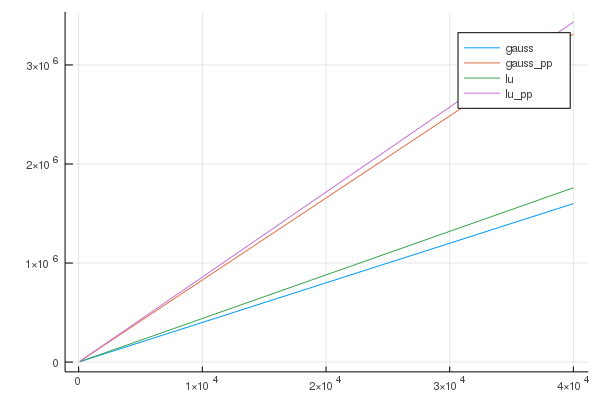
\includegraphics[width=\linewidth]{plot3_ops.png}
  		\caption{Wykres liczby operacji w zależności od $n$}
	\endminipage
\end{figure}

\clearpage
\begin{figure}[!htb]
	\centering
	\minipage{0.7\textwidth}
  		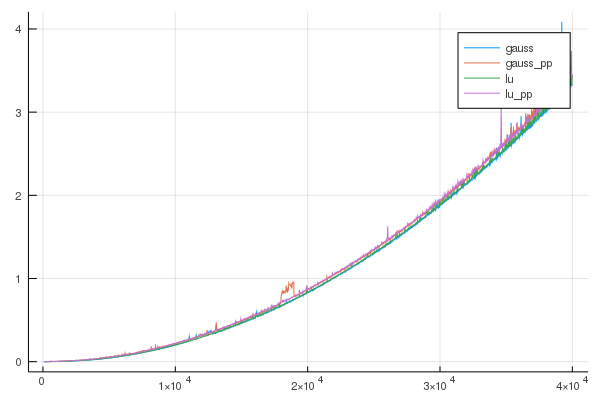
\includegraphics[width=\linewidth]{plot3_time.png}
  		\caption{Wykres czasu rozwiązywania układu w zależności od $n$}
	\endminipage
\end{figure}

\begin{figure}[!htb]
	\centering
	\minipage{0.7\textwidth}
  		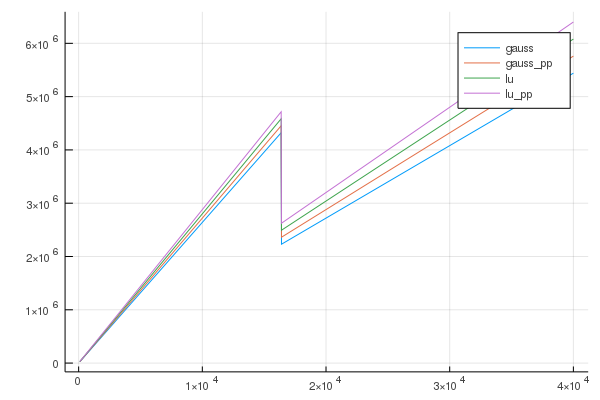
\includegraphics[width=\linewidth]{plot3_mem.png}
  		\caption{Wykres zaalokowanej pamięci w zależności od $n$}
	\endminipage
\end{figure}

\subsubsection*{Obserwacje i wnioski}
Na wykresie liczby operacji można zaobserwować liniową złożoność wszystkich algorytmów, co potwierdza wymaganą złożoność algorytmu $O(n)$. Zgodnie z oczekiwaniami, metody z wyborem elementu głównego wymagały większej liczby operacji. Również metody z wcześniej obliczonym rozkładem \textbf{LU} wymagały większej liczby operacji niż eliminacja bez rozkładu. 

Patrząc na wykres czasu od $n$ możemy zauważyć, że wzrasta on kwadratowo względem $n$. Wynika to z czasu dostępu do elementu w macierzy, gdyby czas ten był stały, czas wzrastałby liniowo względem $n$. 

Patrząc na wykres zaalokowanej pamięci dla poszczególnych wykresów, możemy zauważyć, ze metody z wyborem elementu głównego zajmują więcej pamięci, ze względu na konieczność pamiętania tablicy $p$. Metody z rozkładem \textbf{LU} również wymagają większej ilości pamięci, ze względu na konieczność pamiętania przejściowego wektora $y$.

Obserwując wynikowe wektory $x$, które podczas testów były zapisane do plików, można było dostrzec, że składowe dla algorytmów z wyborem elementów głównych były nieznacznie bliższe wartości $1$, co wskazuje na większą dokładność algorytmu. Zatem jeśli dokładność algorytmu jest dla nas ważniejsza niż szybkość, należy użyć algorytmów z wyborem elementów głównych. Algorytm ten również należy wybrać jeśli na diagonali znajdują się zera.

Głównym wnioskiem płynącym z eksperymentu jest fakt, że znając specyfikację danych wejściowych często możemy w łatwy sposób zmodyfikować algorytm, znacznie zwiększając szybkość jego działania.

\end{document}